\documentclass[tikz]{standalone}
\usepackage{pgfplots}
\pgfplotsset{compat=1.15}
\usepackage{mathrsfs}
\usetikzlibrary{arrows,calc}
\usepackage{tkz-euclide}

\pagestyle{empty}

\definecolor{AngleClr}{rgb}{0,0.39215686274509803,0}
\definecolor{ShapeClr}{rgb}{0.6,0.2,0}

\begin{document}

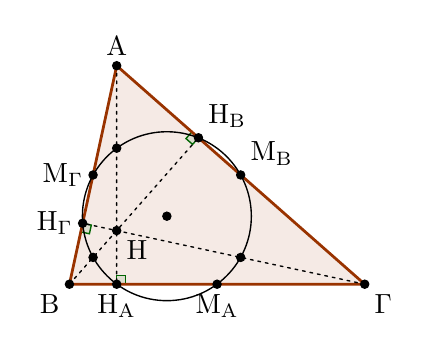
\begin{tikzpicture}[scale=.75]
\tkzSetUpLine[line width=1pt,color=black]
\tkzSetUpPoint[fill=black]

\tkzDefPoints{0/0/B,0.8/3.7/A,5/0/C}

\tkzDefMidPoint(B,C) \tkzGetPoint{MA}
\tkzDefMidPoint(A,C) \tkzGetPoint{MB}
\tkzDefMidPoint(B,A) \tkzGetPoint{MC}


\tkzDefTriangleCenter[circum](MA,MB,MC) \tkzGetPoint{O}
\tkzDefTriangleCenter[ortho](A,B,C) \tkzGetPoint{H}

\tkzDefMidPoint(A,H) \tkzGetPoint{MMA}
\tkzDefMidPoint(B,H) \tkzGetPoint{MMB}
\tkzDefMidPoint(C,H) \tkzGetPoint{MMC}

\tkzDefPointBy[projection = onto B--C](H) \tkzGetPoint{HA}
\tkzDefPointBy[projection = onto A--C](H) \tkzGetPoint{HB}
\tkzDefPointBy[projection = onto A--B](H) \tkzGetPoint{HC}

\tkzFillPolygon[fill=ShapeClr,fill opacity=0.1](A,B,C)

\tkzMarkRightAngles[line width=0.5pt, size=.15,color=AngleClr,fill=AngleClr,fill opacity=0.1](A,HA,C B,HB,A C,HC,B)

\tkzDrawPolygon[color=ShapeClr](A,B,C)

\tkzDrawSegments[line width=0.5pt,color=black,dashed,dash pattern=on 1pt off 1.75pt](A,HA B,HB C,HC)

\tkzDrawCircle[color=black,line width=0.5pt](O,HA)

\tkzDrawPoints[size=3](A,B,C,HA,HB,HC,MA,MB,MC,MMA,MMB,MMC,O,H)
\tkzLabelPoint[above](A){$\mathrm{A}$}
\tkzLabelPoint[below left](B){$\mathrm{B}$}
\tkzLabelPoint[below right](C){$\mathrm{\Gamma}$}

\tkzLabelPoint[below](MA){$\rm M_A$}
\tkzLabelPoint[above right](MB){$\rm M_B$}
\tkzLabelPoint[left](MC){$\rm M_\Gamma$}

\tkzLabelPoint[below](HA){$\rm H_A$}
\tkzLabelPoint[above right](HB){$\rm H_B$}
\tkzLabelPoint[left](HC){$\rm H_\Gamma$}

\tkzLabelPoint[below right](H){$\rm H$}

\end{tikzpicture}
\end{document}
